\documentclass[conference]{IEEEtran}
\IEEEoverridecommandlockouts

\usepackage{cite}
\usepackage{amsmath,amssymb,amsfonts}
\usepackage{graphicx}
\usepackage{textcomp}
\usepackage{xcolor}
\usepackage{booktabs}
\usepackage[hyphens]{url}
\usepackage{hyperref}
\hypersetup{pdftitle={Who Patches the Lightning Network? Release Lines from Gossip, Node Platforms and Security
Advisories, 2023-2026}, pdfauthor={Saurabh Kumar}}

% every number quoted in the text, generated by src/05_supporting_numbers.py
% Generated by src/05_supporting_numbers.py — do not edit by hand.
\newcommand{\ByNinetyCLNAll}{35}
\newcommand{\ByNinetyCLNLarge}{38}
\newcommand{\ByNinetyCLNSmall}{33}
\newcommand{\ByNinetyLNDAll}{50}
\newcommand{\ByNinetyLNDLarge}{53}
\newcommand{\ByNinetyLNDSmall}{42}
\newcommand{\ByYearCLNAll}{77}
\newcommand{\ByYearCLNLarge}{78}
\newcommand{\ByYearCLNSmall}{71}
\newcommand{\ByYearLNDAll}{76}
\newcommand{\ByYearLNDLarge}{82}
\newcommand{\ByYearLNDSmall}{65}
\newcommand{\ClearWaveDay}{8~August~2026}
\newcommand{\ClearWaveLine}{0.21}
\newcommand{\ClearWaveNodes}{114}
\newcommand{\ClearWaveTor}{26}
\newcommand{\CohortClnConnectd}{190}
\newcommand{\CohortClnGossipd}{524}
\newcommand{\CohortEndClnConnectd}{2026-10-13}
\newcommand{\CohortEndClnGossipd}{2026-10-13}
\newcommand{\CohortEndLLBatch}{2026-10-13}
\newcommand{\CohortEndLndSweeper}{2026-04-03}
\newcommand{\CohortLLBatch}{550}
\newcommand{\CohortLeftClnConnectd}{59}
\newcommand{\CohortLeftClnGossipd}{170}
\newcommand{\CohortLeftLLBatch}{108}
\newcommand{\CohortLeftLndSweeper}{356}
\newcommand{\CohortLndSweeper}{1{,}284}
\newcommand{\CohortStillClnConnectd}{60}
\newcommand{\CohortStillClnGossipd}{111}
\newcommand{\CohortStillLLBatch}{388}
\newcommand{\CohortStillLndSweeper}{703}
\newcommand{\CohortUpClnConnectd}{71}
\newcommand{\CohortUpClnGossipd}{243}
\newcommand{\CohortUpLLBatch}{54}
\newcommand{\CohortUpLndSweeper}{225}
\newcommand{\DataFirstDay}{20230508}
\newcommand{\DataUsableDays}{814}
\newcommand{\ExpCapClnConnectdCutoff}{2.4}
\newcommand{\ExpCapClnConnectdDisc}{20.2}
\newcommand{\ExpCapClnConnectdSixty}{3.1}
\newcommand{\ExpCapClnGossipdCutoff}{12.7}
\newcommand{\ExpCapClnGossipdDisc}{57.8}
\newcommand{\ExpCapClnGossipdSixty}{15.6}
\newcommand{\ExpCapLLBatchCutoff}{6.3}
\newcommand{\ExpCapLLBatchDisc}{6.4}
\newcommand{\ExpCapLLBatchSixty}{6.4}
\newcommand{\ExpCapLndSweeperCutoff}{6.3}
\newcommand{\ExpCapLndSweeperDisc}{12.1}
\newcommand{\ExpCapLndSweeperSixty}{9.9}
\newcommand{\ExpClnConnectdCutoff}{12.5}
\newcommand{\ExpClnConnectdDisc}{23.8}
\newcommand{\ExpClnConnectdSixty}{13.7}
\newcommand{\ExpClnGossipdCutoff}{24.2}
\newcommand{\ExpClnGossipdDisc}{66.6}
\newcommand{\ExpClnGossipdSixty}{29.0}
\newcommand{\ExpLLBatchCutoff}{12.5}
\newcommand{\ExpLLBatchDisc}{14.9}
\newcommand{\ExpLLBatchSixty}{12.9}
\newcommand{\ExpLndSweeperCutoff}{12.5}
\newcommand{\ExpLndSweeperDisc}{27.7}
\newcommand{\ExpLndSweeperSixty}{22.3}
\newcommand{\FirstSeenLndMax}{174}
\newcommand{\FirstSeenLndMin}{53}
\newcommand{\FirstSeenLndNineteen}{174}
\newcommand{\FirstSeenLndTwenty}{116}
\newcommand{\FirstSeenLndTwentyOne}{80}
\newcommand{\FixToDiscClnConnectd}{320}
\newcommand{\FixToDiscClnGossipd}{90}
\newcommand{\FixToDiscLLBatch}{446}
\newcommand{\FixToDiscLndSweeper}{196}
\newcommand{\FixToDiscMedian}{256}
\newcommand{\FleetCutoffNodes}{566}
\newcommand{\FleetCutoffShare}{14}
\newcommand{\FleetFirstDay}{20~June~2025}
\newcommand{\FleetPeakCap}{1.3}
\newcommand{\FleetPeakDay}{7~December~2025}
\newcommand{\FleetPeakNodes}{1{,}781}
\newcommand{\FleetPeakShare}{28}
\newcommand{\FleetPeakTotalCap}{8{,}300}
\newcommand{\FleetWaveDay}{9~December~2025}
\newcommand{\FleetWaveNodes}{327}
\newcommand{\MedianCLNAll}{137}
\newcommand{\MedianCLNLarge}{123}
\newcommand{\MedianCLNSmall}{161}
\newcommand{\MedianLNDAll}{90}
\newcommand{\MedianLNDLarge}{79}
\newcommand{\MedianLNDSmall}{142}
\newcommand{\NAdvRows}{23}
\newcommand{\NAdvTotal}{30}
\newcommand{\NAnchorCLN}{117}
\newcommand{\NAnchorClient}{797}
\newcommand{\NAnchorLND}{664}
\newcommand{\NLiveLndCutoff}{3{,}462}
\newcommand{\NOldLndChan}{2{,}689}
\newcommand{\NOldLndLive}{434}
\newcommand{\NVerLines}{11}
\newcommand{\NVerNodeDays}{15{,}549}
\newcommand{\NVerNodeLines}{136}
\newcommand{\NVerNodeLinesExact}{132}
\newcommand{\NVerNodes}{124}
\newcommand{\NWaves}{9}
\newcommand{\NWavesTor}{8}
\newcommand{\ORBehind}{0.19}
\newcommand{\ORCapacity}{1.11}
\newcommand{\ORChannels}{1.15}
\newcommand{\ORDefaultColor}{1.08}
\newcommand{\OROld}{1.01}
\newcommand{\ORTor}{1.59}
\newcommand{\PctCohortStillClnConnectd}{32}
\newcommand{\PctCohortStillClnGossipd}{21}
\newcommand{\PctCohortStillLLBatch}{71}
\newcommand{\PctCohortStillLndSweeper}{55}
\newcommand{\PctIntervalNarrow}{86}
\newcommand{\PctOldLndLive}{12.5}
\newcommand{\PctOldLndNaive}{42.3}
\newcommand{\PctPreCLN}{0.0}
\newcommand{\PctPreLND}{0.1}
\newcommand{\PctStrictMultiCLN}{47}
\newcommand{\PctStrictMultiLND}{11}
\newcommand{\PctUnrecCLN}{0.1}
\newcommand{\PctUnrecLND}{1.0}
\newcommand{\PctVerLikely}{98.2}
\newcommand{\PctVerMaxOperator}{5}
\newcommand{\PctVerStrict}{99.99}
\newcommand{\PrecCLN}{98.3}
\newcommand{\PrecLND}{100.0}
\newcommand{\RateClnConnectdAfter}{20.0}
\newcommand{\RateClnConnectdBefore}{8.3}
\newcommand{\RateClnGossipdAfter}{24.0}
\newcommand{\RateClnGossipdBefore}{5.8}
\newcommand{\RateLLBatchAfter}{6.2}
\newcommand{\RateLLBatchBefore}{6.9}
\newcommand{\RateLndSweeperAfter}{6.5}
\newcommand{\RateLndSweeperBefore}{5.8}
\newcommand{\RecCLN}{99.1}
\newcommand{\RecLND}{96.4}
\newcommand{\TFiftyCapLndEighteen}{41}
\newcommand{\TFiftyCapLndNineteen}{69}
\newcommand{\TFiftyCapLndTwenty}{127}
\newcommand{\TFiftyCapLndTwentyOne}{75}
\newcommand{\TFiftyClnMax}{216}
\newcommand{\TFiftyClnMin}{66}
\newcommand{\TFiftyLndMax}{88}
\newcommand{\TFiftyLndMin}{72}
\newcommand{\TFiftyLndNineteen}{76}
\newcommand{\TFiftyLndTwenty}{88}
\newcommand{\TFiftyLndTwentyOne}{72}
\newcommand{\TFiftyLndTwentyWithFleet}{54}
\newcommand{\TorBaseMax}{73}
\newcommand{\TorBaseMin}{60}
\newcommand{\WaveMaxDays}{69}
\newcommand{\WaveMaxNodes}{252}
\newcommand{\WaveMedianAge}{471}
\newcommand{\WaveMedianCap}{0.051}
\newcommand{\WaveMinDays}{23}
\newcommand{\WaveMinNodes}{114}
\newcommand{\WaveOtherCap}{0.053}
\newcommand{\WaveTorMax}{93}
\newcommand{\WaveTorMin}{76}


\begin{document}

\title{Who Patches the Lightning Network?\\
{\LARGE Release Lines from Gossip, Node Platforms and Security Advisories, 2023--2026}}

\author{
\IEEEauthorblockN{Saurabh Kumar}
\IEEEauthorblockA{Bitcoin Data Labs\\
sorukumar@bitcoindatalabs.org}
}

\maketitle
\thispagestyle{plain}
\pagestyle{plain}

% ==========================================================================================
\begin{abstract}
Every Lightning implementation disclosed security vulnerabilities in 2026, and every advisory told operators to
upgrade. Whether they do has never been measured, because Lightning gossip carries no software version. We show that
the release line of a public node can be read from the feature bits it announces: matched against the source of every
release of LND, Core Lightning, Eclair and LDK, the inferred range contains the true line on \PctVerStrict\% of
\NVerNodeDays{} node-days of nodes that state their version, and the most likely line is exact on \PctVerLikely\%.
Applying it to \DataUsableDays{} daily snapshots of the public graph from 2023 to 2026, we find that half of the
LND nodes on an older line upgrade within \MedianLNDAll{} days of a release, in waves consistent with node platforms
pushing updates, while small nodes and nodes that skipped earlier releases lag far behind. One operator ran up to
\FleetPeakNodes{} public LND nodes, \FleetPeakShare\% of all live LND nodes, with about one bitcoin between them.
For \NAdvTotal{} LND and CLN advisories, fixes shipped a median \FixToDiscMedian{} days before disclosure. LND's
disclosures did not change how fast operators left vulnerable releases: two months after Lightning Labs' August~2026
batch, \PctCohortStillLLBatch\% of the nodes exposed at disclosure still ran an affected release. CLN's disclosures
of July~2026 raised the monthly rate at which nodes left vulnerable releases two- to fourfold. Exposure measured by
capacity is small; by node count, it depends on how one counts a single operator's fleet.

\end{abstract}

\begin{IEEEkeywords}
Lightning Network, Bitcoin, patch deployment, vulnerability disclosure, node platforms, software versions,
measurement, gossip
\end{IEEEkeywords}

% ==========================================================================================
\section{Introduction}
\label{sec:intro}

The Lightning Network is a payment network built on Bitcoin. Its nodes run open-source software and hold their
operators' funds in payment channels, so a flaw in that software can put those funds at risk. Between July and
October~2026, every major Lightning implementation disclosed security vulnerabilities. Lightning
Labs published ten LND advisories on a single day~\cite{lightninglabs2026aug} and eight more a month
later~\cite{lightninglabs2026sep}; Core Lightning (CLN) asked operators who could not upgrade to restart their nodes
offline~\cite{coreln2026offline}; Eclair and LDK shipped security releases. Each advisory ends with the same advice:
upgrade. Whether operators do, and how fast, decides how long a disclosed vulnerability stays exploitable, and by
October CLN's maintainers reported attacks on unpatched nodes~\cite{coreln2026attacks}. For web servers, browsers and
Bitcoin and Ethereum full nodes, how fast operators patch has been measured for two decades
\cite{arbaugh2000windows,rescorla2003securityholes,frei2009firefox,durumeric2014heartbleed,kim2018ethereum}. For the
Lightning Network it has not, because Lightning gossip carries no software version: earlier studies could tell which
implementation a node runs~\cite{zabka2021nodeclassification,espinasa2024decisiontree,kumar2026clientdiversity}, not
which release.

We show that the release can be read from gossip after all, and use it to ask who patches the Lightning Network:
operators on their own schedule, the platforms that package the implementations, or the advisories themselves. Each
release announces a characteristic set of protocol feature bits. From the source of every release of LND, CLN, Eclair
and LDK since 2019 we derive which sets each release can produce, and match them against \DataUsableDays{} daily
snapshots of the public graph taken by our own node from May~2023 to October~2026. The answer is that the network
patches on release and platform schedules, not on disclosures. Most operators upgrade within months of a release;
the largest movements are platforms shipping a release to all their users at once; and an advisory, published long
after its fix, moves at most the operators who were already close to current. We make four contributions.

\begin{itemize}
\item \textbf{Release-line inference from gossip.} The release line of a public node can be read from its gossip.
A release line is the finest unit gossip separates; patch releases are invisible. Where a node states its version, the
inference is close to exact: on CLN nodes whose alias names the version, the most likely line is right for
\NVerNodeLinesExact{} of \NVerNodeLines{} node--line pairs. LND nodes state no version, so we check three things that
must hold if the inference is right, and all three do: line decreases are \PctDownLND\% of observed line changes, no
LND line released since 2024 was seen on more than \PreRelLndMax{} nodes before its publication, and
\PlatLineMin--\PlatLineMax\% of the nodes that changed line right after a platform shipped a new LND line landed on
the line it shipped (\S\ref{sec:inference}).
\item \textbf{Upgrade dynamics.} Most operators upgrade within months; the ones that lag are small or already behind. Half of the
LND nodes on an older line upgrade within \MedianLNDAll{} days of a release; the smallest quarter of nodes takes
\MedianLNDSmall{}, and a node already more than one line behind has about five times lower odds of moving in any
week. These figures set apart a managed fleet of up to \FleetPeakNodes{} live LND
nodes~\cite{kumar2026clientdiversity}, whose schedule would otherwise dominate them (\S\ref{sec:dynamics}).
\item \textbf{Platforms set the pace.} The largest upgrades are node platforms shipping a release to all their users
at once. Dating the releases of two platforms to the minute from public records, we find that the three largest LND
upgrade waves, \WaveUmbrelMinNodes--\WaveUmbrelMaxNodes{} nodes each, came about a day after the Umbrel app store
published a new LND version, and another followed BTCPay Server's security release. Since June~2025, the 48~hours
after such releases cover \PlatTimeLND\% of the time but hold \PlatShareLND\% of LND upgrades (\S\ref{sec:waves}).
\item \textbf{Disclosure, response and exposure.} Disclosure moved few operators, and mostly those already close to
current. For the \NAdvTotal{} LND and CLN advisories whose fix boundary gossip can see, we measure how many live nodes
and how much capacity stayed exposed; the fixes typically shipped months before disclosure (median \FixToDiscMedian{}
days). For \NResp{} disclosures we test whether exposed nodes left the affected lines faster afterwards. Only CLN's
July~2026 disclosures
raised that rate, by a factor of \RROpClnRecent{} among nodes one line behind; nodes further behind moved when
BTCPay's own advisory had their operators update. No LND disclosure produced a detectable increase: two months after
Lightning Labs' August~2026 batch, \PctCohortStillLLBatch\% of the nodes exposed at disclosure still ran an affected
release. When CLN asked operators who could not upgrade to restart offline, the nodes that went offline were mostly
already patched: \OffCallNewestLeft\% of the nodes on the newest line went offline, against \OffCallBehindLeft\% of
the nodes behind (\S\ref{sec:exposure}).
\end{itemize}

All data behind the figures and tables, and the code, are released. We report aggregates only: no list, ranking or
label of individual nodes by release, platform or exposure.

% ==========================================================================================
\section{Background and Related Work}
\label{sec:background}

\subsection{Gossip and feature bits}
Public Lightning nodes announce themselves and their channels through gossip~\cite{bolt7}. A node's
\texttt{node\_announcement} carries its alias, colour, network addresses and a feature vector: a bit field in which
each pair of bits marks a protocol feature as required (even bit) or optional (odd bit)~\cite{bolt9}. Implementations
set their feature vector from compiled-in defaults, which change when a release adds or retires a feature, plus
whatever options the operator switches on. Gossip carries no version string. A node re-signs its announcement when
it restarts or changes its settings, so a node that upgrades and restarts re-announces with the feature vector of
the new release.

\subsection{Inferring implementations}
Zabka et al.\ classify public nodes into LND, c-lightning and Eclair from default channel parameters, colours and
aliases~\cite{zabka2021nodeclassification,zabka2022empirical}. Their study contains the only prior observation of an
LND upgrade we found: after LND changed its default CLTV delta from 144 to 40 in March~2019, the new value overtook
the old one around mid-December, about nine months later. They name the planning of critical software updates as a
use of implementation inference but do not measure it. Espinasa-Vilarrasa et al.\ infer the implementation from
gossip traffic or from announced feature bits with decision trees~\cite{espinasa2024decisiontree}. Kappos et al.\
note that their gossip snapshots carried no version information, and fell back on owner-reported fields for 370
nodes~\cite{kappos2021privacy}. Our previous paper used feature-bit rules to measure client concentration and the
2026 Core Lightning shutdown~\cite{kumar2026clientdiversity}. All of these stop at the implementation; none infers
which release a node runs.

Longitudinal studies of the Lightning graph cover topology, centralisation and robustness
\cite{rohrer2019discharged,seres2020topological,lin2020secondpath,martinazzi2020evolving,zabka2024centrality},
infrastructure~\cite{casas2021taproot}, privacy~\cite{romiti2021crosslayer}, channel lifecycles
\cite{grotschla2025lifecycle}, gossip convergence~\cite{gogge2023convergence} and, most recently, stability and node
lifetimes~\cite{valko2025geolocated,valko2025stability,valko2026lifetime}. None of them studies software versions.
When Lightning Labs disclosed CVE-2019-12999, they were ``surprised to find many nodes running very old versions''
but published no numbers~\cite{lightninglabs2019cve}.

\subsection{Versions in other blockchain networks}
Bitcoin and Ethereum peers report their software version in the handshake, so crawlers can count versions directly.
Kim et al.\ found 68\% of Geth nodes two or more releases behind and tracked client age against release
dates~\cite{kim2018ethereum}. Neudecker reports that Bitcoin nodes adopt a release mostly in its first two months,
and documents an alternative client that went from zero to more than 700 peers in a
day~\cite{neudecker2019characterization}; Park et al.\ and Eisenbarth et al.\ survey Bitcoin node versions and their
known vulnerabilities~\cite{park2019bitcoinnodes,eisenbarth2021bitcoin}. SRLabs estimated that about 40\% of Parity
nodes were still vulnerable a month after an advisory~\cite{srlabs2019patchgap}. Zcash sidesteps slow upgrades by
expiring old releases at network upgrades~\cite{daniel2019mapz}. The Lightning Network offers neither a version
string to count nor a forced expiry.

\subsection{Patch deployment}
The window of vulnerability, from disclosure to patch, was framed by Arbaugh et al.~\cite{arbaugh2000windows}.
Rescorla probed servers affected by the OpenSSL vulnerabilities of 2002 and found more than two thirds still
vulnerable two weeks after disclosure~\cite{rescorla2003securityholes}. Frei et al.\ showed that automatic
updates dominate how fast a client population patches~\cite{frei2009firefox}, Durumeric et al.\ followed Heartbleed
across the Internet~\cite{durumeric2014heartbleed}, and Nappa et al.\ modelled patch deployment with survival
analysis~\cite{nappa2015clones}; Li and Paxson measured the life cycle of security fixes from the code
side~\cite{li2017patches}. We bring this lens to a network where versions must first be inferred, and where a
release is often fixed months or years before the vulnerability is disclosed.

% ==========================================================================================
\section{Data and Vantage Point}
\label{sec:data}

\paragraph{Gossip snapshots}
We take a daily dump of the public graph (\texttt{describegraph}) from our own LND node and keep, per day, every
node announcement (feature bits, alias, colour, addresses, last-update time) and every channel direction (the policy
a node sets for forwarding towards its peer, with capacity, the \emph{disabled} flag and last-update time). The
snapshots run from May~2023 to the data cutoff of 13~October~2026. A per-day quality check discards dumps that
are partial (fewer than half the channels of their period), stale (fewer than half the channels updated within two
weeks) or error responses written while the node's wallet was locked; \DataUsableDays{} days remain. Daily coverage is
dense from November~2023, with gaps in May--June~2024 (partial dumps), August~2024 and January--May~2025 (wallet
locked after restarts). Upgrade times observed across a gap are known only to lie inside it; we treat them as
interval-censored (\S\ref{sec:dynamics}).

\paragraph{Vantage}
All snapshots are one node's view. LND prunes channels that have not been updated for about two weeks, and our
view widened in July~2024 (from about 8.4k to 11--13k nodes with channels), after the node's own peer set grew. We
compare levels within a period and report shares, which are less sensitive to the view; in particular, the few
live nodes on releases from before 2021 appear only from July~2024. Only announced (public) nodes are visible:
mobile wallets and services behind unannounced channels, where much of LDK and Eclair runs, are not.

\paragraph{Who is still there}
Nodes that stop running do not leave the graph at once: their peers mark the channels towards them disabled, and
the channels stay announced until they are closed or pruned. An offline node cannot announce anything, so liveness
must be read from its peers' side~\cite{kumar2026clientdiversity}. We call a node \emph{live} on a day when at least
one channel direction towards it, set by a peer, is enabled and was updated in the previous 14~days; its \emph{live
capacity} is the capacity of those channels. We also report 7- and 28-day variants. The distinction matters. On
the cutoff day, \NOldLndChan{} LND nodes with channels (outside the managed fleet of \S\ref{sec:dynamics})
announced a release older than 0.19, but only
\NOldLndLive{} of them were live; counting every announced node would put the share of LND nodes on those releases
at \PctOldLndNaive\%, against \PctOldLndLive\% of live nodes.

% ==========================================================================================
\section{Inferring Release Lines from Gossip}
\label{sec:inference}

\subsection{Release lines}
We built a table of the \texttt{node\_announcement} feature bits of every release of the four implementations from
their source at each release tag: LND 0.7--0.21.4, Core Lightning (CLN) 0.8.2--26.06.9, Eclair 0.3--0.14.3 and LDK
0.0.113--0.2.7. For each release we record the bits it sets by default, the bits an operator can add through
options, flags, plugins or known custom extensions, and the default bits an operator can switch off; each entry
cites the source file it comes from. A release's date is its publication date (GitHub release page; crates.io for
LDK), the day operators could install it. Consecutive releases with identical defaults form a \emph{release line}, the
finest unit gossip can resolve: LND has 10 lines from 0.8 to 0.21, CLN 13, Eclair 13 and LDK 6. Some lines are
single minor releases (LND 0.18, 0.19, 0.20, 0.21); others span several (LND 0.15.1--0.17; LDK 0.0.120--0.1 covers
January~2024 to December~2025). Patch releases never change the defaults, so a patch level is never visible.

For a node with feature set $B$, a line $\ell$ with defaults $D_\ell$, optional bits $O_\ell$ and removable bits
$R_\ell$ is \emph{consistent} when $D_\ell \setminus R_\ell \subseteq B \subseteq D_\ell \cup O_\ell$. The
\emph{strict range} is every consistent line released by the day of observation; it contains the running line under
any non-developer configuration. The \emph{likely line} is the consistent line that needs the fewest non-default
bits among the lines released by the day the node's current feature set first appeared. Dating the inference to
that day matters: a node cannot run a line that did not exist when it began announcing its bits, and without it a
new release would relabel every node whose existing bits happen to fit the new line (233 CLN nodes running 24.05 with
the onion-message option would have ``upgraded'' to 24.08 on its release day). A set consistent only with lines not
yet released is a pre-release build; a set consistent with no line is unrecognised.

\subsection{Implementation}
Release lines are defined per implementation, so the implementation comes first. We revise the feature-bit rules of
our previous paper~\cite{kumar2026clientdiversity}: LND-only bits (2023, 31) and Eclair-only bits (37, or 29
with 61) are decisive; a set with bits 11 and 39 or 43 is CLN when bit 5 is set and Eclair otherwise; 39, 43 or 63
without 11 is LDK. The CLN--Eclair split now uses bit 5 (\texttt{upfront\_shutdown\_script}), which every CLN
release sets, instead of keysend (bit 55), which operators can switch off. New in this paper, the release table
itself is evidence. When a set is consistent with the
lines of exactly one implementation, that implementation is assigned, which recovers releases older than the
distinguishing bits, such as LND 0.8--0.11 and CLN before 23.05; and when a bit rule names an implementation that
has no release producing the set while exactly one other implementation does, the table wins. Weak signals (LND's
default colour or alias, default CLTV deltas) label the remaining nodes with low confidence, and only operator-attributed
and high-confidence labels receive a release line. Announcements that are not visible on a day (last update~0)
carry the node's previous feature set forward.

\subsection{Validation}
\label{sec:validation}
\paragraph{Implementation}
\NAnchorClient{} nodes name their implementation in their alias (``\ldots{}[LND]'', ``\ldots{}-CLN'', ``eclair'',
``ldk-node''); LND's default alias is excluded because the rules use it. On the latest day each was announced with
channels, the labels reach precision \PrecLND\% and recall \RecLND\% for LND (\NAnchorLND{} nodes) and precision
\PrecCLN\% and recall \RecCLN\% for CLN (\NAnchorCLN{} nodes) (Table~\ref{tab:validation}). The misses are almost
all low-confidence labels, which receive no release line.

\paragraph{Release line}
CLN built in developer mode puts the version into the default alias (e.g.\ \texttt{YELLOWWATER-v25.09}); the alias
follows the binary, so it is correct on every day the node is announced. Over \NVerNodeDays{} announced node-days of
\NVerNodes{} such nodes on \NVerLines{} lines (no operator above \PctVerMaxOperator\% of node-days), the strict range
contains the stated line on \PctVerStrict\% of node-days and the likely line is exact on \PctVerLikely\%
(Fig.~\ref{fig:validation}). Node-days of one node are not independent, so the node is the better unit: of the
\NVerNodeLines{} combinations of node and stated line, \NVerNodeLinesExact{} are exact on every day
(\PctNodeLineExact\%, 95\% CI \NodeLineCILo--\NodeLineCIHi\%). The misses are a 24.05 node with the onion-message
option, which makes it identical to 24.08; a 25.02.1 node and a 23.11.1 node whose switched-off options make them look
one line older; and a single day of a release candidate.

\paragraph{Checks without ground truth}
No LND node in our data states its version in its alias, so for LND, where most of our dynamics are measured, we rely
on checks that a wrong release table would fail. First, operators rarely return to an older release, while a noisy
inference would make nodes flicker between lines: among consecutive observations of live nodes, the likely line
decreases in \PctDownLND\% of line changes for LND (against \NUpLND{} increases) and in \PctDownCLN\% for CLN. Second,
a line assigned the wrong bits would show nodes on it long before its release: each LND line released since 2024 was
seen on at most \PreRelLndMax{} nodes before its publication, against \PostRelLndMin--\PostRelLndMax{} in its first
90~days. Third, a check from outside gossip: a platform that ships a new LND version moves its nodes to a known line
(\S\ref{sec:waves}). Of the \NPlatLineChanges{} line changes whose new announcement was signed within 48~hours after
one of the four platform releases that introduced a new LND line, \PlatLineMin--\PlatLineMax\% landed
on the line that release shipped.

\paragraph{What gossip cannot resolve}
Among live nodes with a release line, the strict range spans more than one line on \PctStrictMultiLND\% of LND and
\PctStrictMultiCLN\% of CLN node-days in 2026, because options let an older line imitate a newer one; the likely line
is unique on all of them. Unrecognised sets are \PctUnrecLND\% (LND) and \PctUnrecCLN\% (CLN) of node-days,
and pre-release builds about \PctPreLND\% of LND node-days. Three limits remain. Patch releases are invisible.
A node that upgrades without restarting, or whose new announcement does not reach us, keeps its old bits. Developer
overrides and forks can imitate any set. The first two bias exposure upward, the third in either direction; none
can be measured from gossip alone, which is why we report the strict and likely ranges side by side.

\begin{figure}[t]
\centering
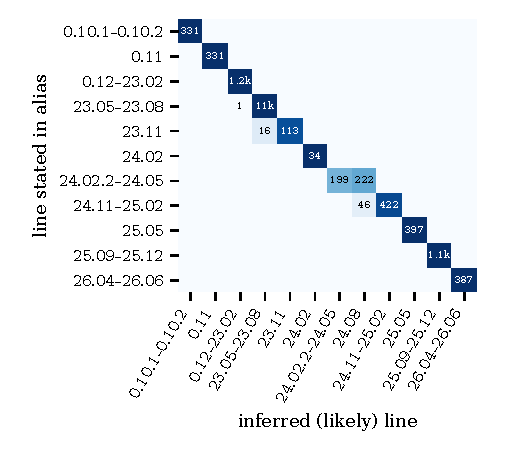
\includegraphics[width=\columnwidth]{figures/fig2_version_validation.pdf}
\caption{Release line stated in CLN developer aliases (rows) against the likely line inferred from feature bits
(columns), in node-days. Shading is the row share.}
\label{fig:validation}
\end{figure}

\begin{table}[t]
\centering\small
\caption{Validation against self-identifying aliases. Top: client labels of 797 nodes whose alias names their implementation. Bottom: release lines of CLN nodes whose alias states the running version, graded on every announced node-day.}
\label{tab:validation}
\begin{tabular}{lrrr}
\toprule
Client & Nodes & Precision (\%) & Recall (\%) \\
\midrule
LND & 664 & 100.0 & 96.4 \\
CLN & 117 & 98.3 & 99.1 \\
Eclair & 9 & 58.3 & 77.8 \\
LDK & 7 & 100.0 & 100.0 \\
\midrule
\multicolumn{3}{l}{CLN nodes / lines with a stated version} & 124 / 11 \\
\multicolumn{3}{l}{Node-days graded} & 15,549 \\
\multicolumn{3}{l}{Strict range contains the stated line (\%)} & 99.99 \\
\multicolumn{3}{l}{Likely line equals the stated line (\%)} & 98.2 \\
\multicolumn{3}{l}{Node--line pairs exact on every day} & 132 / 136 \\
\multicolumn{3}{l}{\quad 95\% CI (\%)} & [93, 99] \\
\bottomrule
\end{tabular}
\end{table}


% ==========================================================================================
\section{How Lightning Nodes Upgrade}
\label{sec:dynamics}

\subsection{Adoption of new release lines}
Fig.~\ref{fig:linemix} shows the release-line mix of live LND and CLN nodes. Each new LND line displaces its
predecessor within a few months but leaves a tail: at the cutoff, \PctOldLndLive\% of live LND nodes were still on a
line older than 0.19, released in May~2025. New lines reached half of live LND nodes \TFiftyLndMin--\TFiftyLndMax{}
days after release (Fig.~\ref{fig:adoption}); half of live capacity moved as fast or faster for 0.18 and 0.19
(\TFiftyCapLndEighteen{} and \TFiftyCapLndNineteen{} days) but more slowly for 0.20 (\TFiftyCapLndTwenty{} days).
Counting the fleet as independent nodes would put LND 0.20 at 50\% of nodes after \TFiftyLndTwentyWithFleet{} days
instead of \TFiftyLndTwenty{}. CLN lines took \TFiftyClnMin--\TFiftyClnMax{} days. Every LND line from 0.18 on was
announced by a few nodes \FirstSeenLndMin--\FirstSeenLndMax{} days before its release: developers and early adopters
running unreleased builds on mainnet.

\begin{figure*}[t]
\centering
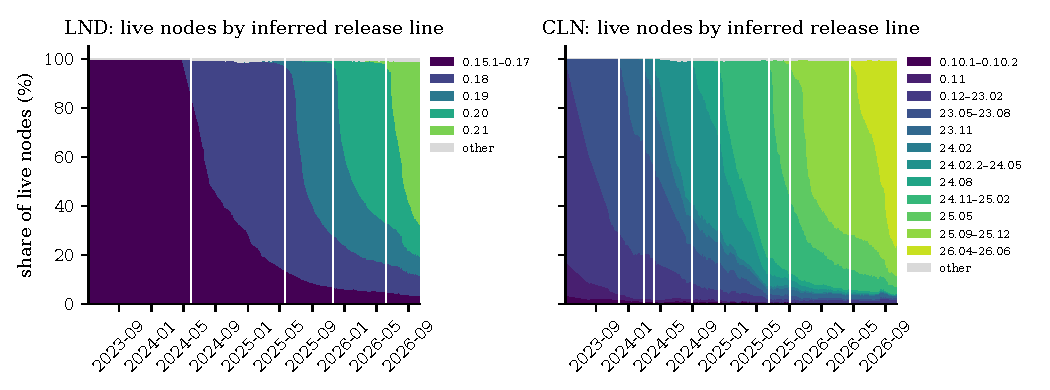
\includegraphics[width=\textwidth]{figures/fig1_line_mix.pdf}
\caption{Live LND and CLN nodes by inferred release line (likely line), excluding the managed fleet. White lines mark
releases. Lines under 2\% of nodes throughout are grouped as ``other''.}
\label{fig:linemix}
\end{figure*}

\begin{figure*}[t]
\centering
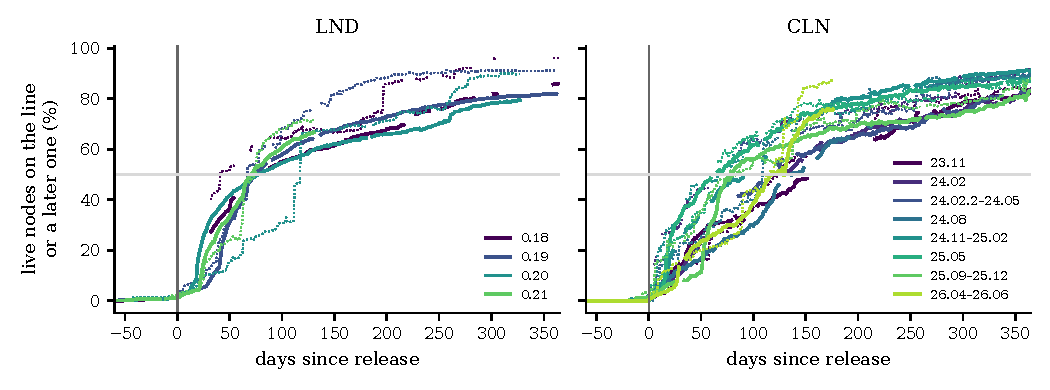
\includegraphics[width=\textwidth]{figures/fig3_adoption.pdf}
\caption{Share of live nodes (solid) and of their live capacity (dotted) on each release line or a later one, by
days since the line's release. Lines are broken across snapshot gaps longer than three days.}
\label{fig:adoption}
\end{figure*}

\subsection{Time to upgrade}
Adoption curves mix upgrades with nodes arriving and leaving. To follow operators, we take every node that is live
on an older line on the release day of LND 0.19, 0.20 or 0.21 or of a CLN line from 23.11 on, and measure the time
until it is first seen on the new line or a later one. Snapshot gaps leave the upgrade day inside an interval (for
\PctIntervalNarrow\% of LND upgrades it is at most two days wide); nodes that stop being live before upgrading are
censored at their last live day. The share upgraded by day $t$ is the nonparametric maximum-likelihood estimate for
interval-censored data~\cite{turnbull1976empirical}. Half of the LND nodes upgraded within \MedianLNDAll{} days and
\ByYearLNDAll\% within a year; for CLN the median is \MedianCLNAll{} days. Size matters at the bottom: the smallest
quarter of LND nodes by live capacity took a median \MedianLNDSmall{} days, the largest quarter \MedianLNDLarge{}
(Fig.~\ref{fig:ttu}).

Table~\ref{tab:hazard} fits a discrete-time model of the weekly probability of upgrading for LND. Larger nodes
upgrade sooner (odds ratio \ORCapacity{} per tenfold capacity, \ORChannels{} per tenfold channel count), and so do
Tor-only nodes (\ORTor{}), which make up most of the platform waves of \S\ref{sec:waves}. A node more than one line
behind when the release ships is far less likely to move (\ORBehind{}): the tail is made of nodes that skipped releases before.
Nodes with LND's default colour are no slower (\ORDefaultColor{}), and nodes seen before 2024 upgrade at the same
rate as newer ones (\OROld{}).

\begin{figure*}[t]
\centering
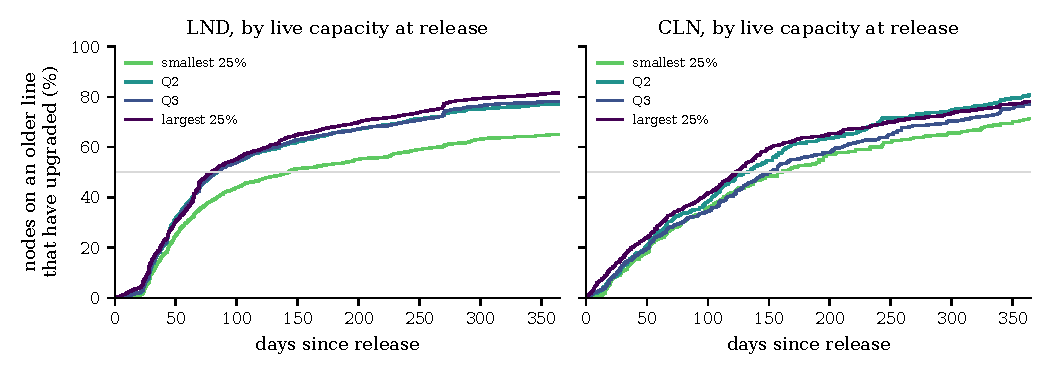
\includegraphics[width=\textwidth]{figures/fig4_time_to_upgrade.pdf}
\caption{Share of nodes that were live on an older line at a release and have since been seen on the new line or a
later one, by quartile of live capacity at the release (Turnbull estimate; LND 0.19--0.21, CLN 23.11--26.04).}
\label{fig:ttu}
\end{figure*}

\begin{table}[t]
\centering\small
\caption{What predicts upgrading: discrete-time logit on node-weeks after each LND release (week and release fixed effects; standard errors clustered by node). Odds ratios with 95\% CI.}
\label{tab:hazard}
\begin{tabular}{lrr}
\toprule
Covariate & Odds ratio & 95\% CI \\
\midrule
Capacity ($\times$10) & 1.11 & [1.07, 1.16] \\
Channels ($\times$10) & 1.15 & [1.06, 1.24] \\
Tor-only & 1.59 & [1.50, 1.69] \\
LND default colour & 1.08 & [1.03, 1.14] \\
Seen before 2024 & 1.01 & [0.96, 1.07] \\
$>$1 line behind & 0.19 & [0.18, 0.21] \\
\midrule
Nodes / node-weeks & \multicolumn{2}{r}{7,218 / 228,254} \\
\bottomrule
\end{tabular}
\end{table}


% ==========================================================================================
\section{Platforms Set the Pace}
\label{sec:waves}

\subsection{Dating platform releases}
Gossip does not name the platform a node runs on, but the signing time of a node's first announcement on a new line
can be set against platform releases dated to the minute. For Umbrel we take the merge time of every pull request
that changed the version of its LND or CLN app from 2024 to the cutoff~\cite{umbrel2026apps}. A BTCPay Server
deployment updates only when its operator runs the update, which installs the LND or CLN version BTCPay pins at that
moment, so its routine version bumps reach nodes over weeks; we take its security release 2.4.2 of 7~August~2026,
which asked every operator to update at once~\cite{btcpay2026advisory}. Start9, RaspiBlitz, myNode and hosted
services publish through channels we cannot date to the day and are not covered.

\subsection{Upgrade waves}
Upgrades arrive in bursts (Fig.~\ref{fig:waves}). We call a day a wave day for a line when more nodes moved to it
than on 99\% of all (day, line) pairs, and merge consecutive wave days on one line into an event. Outside the fleet,
LND had \NWaveEvents{} events of \WaveMinNodes--\WaveMaxNodes{} nodes. None came at the line's release; all came
\WaveMinDays--\WaveMaxDays{} days later. They are real upgrades, not gossip catching up after a gap: in every
event, \WaveMinSignedTwo\% of the nodes had signed their new announcement within two days before we first saw it.

The three largest were set by Umbrel, not by LND. Each followed Umbrel's release of a new LND version (0.19.1, 0.20.0
and 0.21.1), which came \WaveUmbrelDaysMin--\WaveUmbrelDaysMax{} days after LND's own. The timing is Umbrel's: in
each wave, at least \WaveUmbrelSignedMin\% of the \WaveUmbrelMinNodes--\WaveUmbrelMaxNodes{} nodes signed their new
announcement within 48~hours after Umbrel merged the release (median \WaveUmbrelHoursMin--\WaveUmbrelHoursMax{}~hours
after), and at most \WaveUmbrelBeforeMax\% in the 24~hours before. These nodes are far more often Tor-only than the
rest of the network (\WaveUmbrelTorMin--\WaveUmbrelTorMax\%, against \WaveUmbrelBaseMin--\WaveUmbrelBaseMax\% of all
live LND nodes). Even the managed fleet of \S\ref{sec:data} kept Umbrel's schedule: \FleetWaveNodes{} of its nodes
moved to LND 0.20 on \FleetWaveDay{}, \FleetWaveSigned\% of them within 48~hours after Umbrel published 0.20.0, with
the same median lag (\FleetWaveHours{}~hours) as the platform's other users.

A fourth event followed BTCPay Server's security release: \WaveBTCPayNodes{} nodes on \WaveBTCPayDay{},
\WaveBTCPaySigned\% of them signed within 48~hours after it. Unlike the Umbrel waves, these nodes are mostly clearnet
(\WaveBTCPayTor\% Tor-only, against \WaveBTCPayBase\%), and \WaveBTCPayOlder{} of them came from lines older than
0.20, skipping at least one release. They look like operators who had not moved to a newer LND line in months and
did so when the advisory for their merchant software told them to update; that advisory concerned BTCPay itself, not
LND. Of the remaining two events, one (\WaveEarlyNodes{} nodes, \WaveEarlyDay) was signed before Umbrel merged LND
\WaveEarlyVersion{} (\WaveEarlyBefore\% in the 24~hours before), so that release cannot explain it, and one
(\WaveNoneNodes{} nodes, \WaveNoneDay) matches no release we can date. CLN shows the same pattern at its smaller
scale: its one attributed event, \ClnWaveNodes{} nodes on \ClnWaveDay{}, followed Umbrel's release of CLN 26.04.1,
\ClnWaveSigned\% of them within 48~hours.

\begin{figure*}[t]
\centering
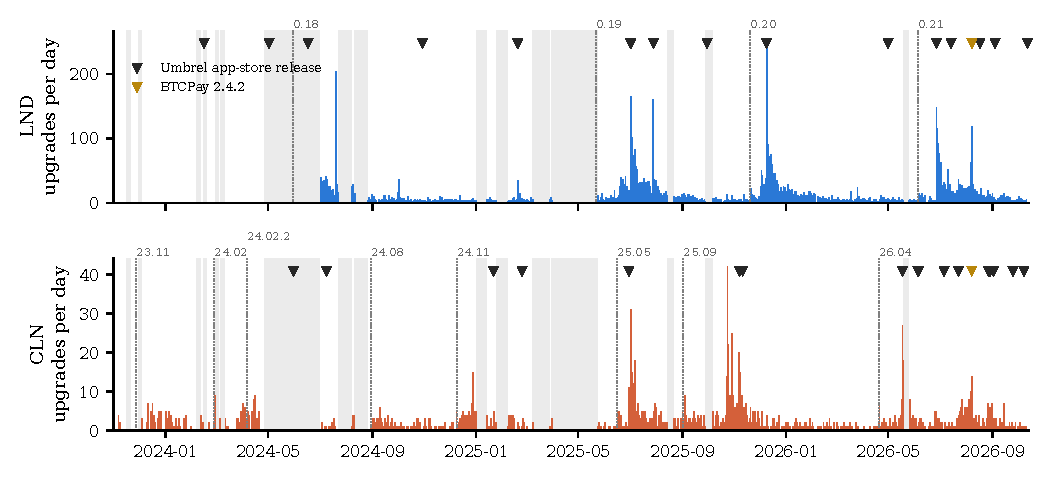
\includegraphics[width=\textwidth]{figures/fig5_waves.pdf}
\caption{Nodes first seen on a newer release line per day, where the upgrade day is known to within two days
(managed fleet excluded). Grey: snapshot gaps; dotted lines: LND and CLN releases; triangles: Umbrel app-store
releases (black) and BTCPay Server's security release 2.4.2 (gold) of that implementation.}
\label{fig:waves}
\end{figure*}

\subsection{Beyond the waves}
Platform releases account for a share of upgrades out of proportion to the time they cover. Since June~2025,
\PlatShareLND\% of LND upgrades whose day is known to within two days were signed within 48~hours after a platform
release that ships the new line, although these windows cover \PlatTimeLND\% of the time; for CLN, \PlatShareCLN\%
against \PlatTimeCLN\%. Since the platforms we cannot date are left out, these shares are lower bounds. The pushes
also check the inference: the nodes that changed line right after a platform shipped a new LND line landed on the
line it shipped (\S\ref{sec:validation}).

% ==========================================================================================
\section{Exposure after Security Advisories}
\label{sec:exposure}

\subsection{Advisories gossip can see}
We collected every public security advisory for LND, CLN, Eclair and LDK from January~2022 to the cutoff (release
notes, Lightning Labs' advisory index, Delving Bitcoin and authors' write-ups), recording the affected versions, the
first fixed release and the disclosure date. An advisory is visible in gossip when its fix boundary coincides with
the start of a release line (LINE), or falls inside a line but leaves whole lines affected or fixed on either side
(PARTIAL, which gives bounds). Fixes inside the newest line, such as CLN 26.06.7--26.06.9 and Eclair 0.14.1--0.14.3,
are patch releases and invisible. Eclair and LDK have too few live public nodes with a known line (about ten Eclair
nodes) for shares to be meaningful, so Table~\ref{tab:advisories} lists the \NAdvRows{} LND and CLN entries,
covering \NAdvTotal{} advisories.

Two clocks run for each advisory. Fixes usually ship long before the vulnerability is disclosed: the median gap
between the first fixed release and disclosure is \FixToDiscMedian{} days, and the six advisories Lightning Labs
published on 11~August~2026 concerned bugs fixed in LND 0.19.0, released \FixToDiscLLBatch{} days earlier. A node
still on an affected line at disclosure has therefore usually skipped a release that was already available for many
months. Exposure is the share of live nodes (excluding the managed fleet) on an affected line, with the share of
their live capacity alongside.

\begin{table*}[t]
\centering\footnotesize
\caption{Advisories whose fix boundary is visible in gossip (LND and CLN). Exposure = share of live nodes of that implementation whose inferred release line is affected, in \%; share of their live capacity in parentheses; for PARTIAL rows (the fix lands inside a line) the bounds are given in brackets at disclosure. Fix$\to$disc.\ = days from the first fixed release to public disclosure. \# = advisories grouped in the row.}
\label{tab:advisories}
\resizebox{\textwidth}{!}{%
\begin{tabular}{lllrlrrrrr}
\toprule
Impl. & Advisory & Class & \# & Fixed in & Fix$\to$disc. & At fix & At disclosure & +60\,d & Cutoff \\
\midrule
CLN & Fake channel DoS (2023-08-23) & PARTIAL & 1 & 23.02 & 175 & -- & -- & 6 (2) & 1 (0) \\
CLN & Replacement cycling (CVE-2023-40234) (2023-10-16) & PARTIAL & 1 & 23.08.1 & 34 & -- & 38 [24--100] (17) & 26 (10) & 2 (0) \\
CLN & BOLT11 parsing bugs, batch 1 (2023-12-08) & PARTIAL & 1 & 23.02 & 282 & -- & 4 [4--95] (2) & 2 (1) & 1 (0) \\
CLN & BOLT11 parsing bugs, batch 2 (2023-12-08) & LINE & 1 & 23.11 & 10 & 99 (100) & 96 (96) & 69 (73) & 3 (0) \\
CLN & funding\_created assertion DoS (2026-05-16) & LINE & 1 & 25.09 & 256 & 98 (97) & 29 (24) & 24 (21) & 12 (2) \\
CLN & connectd queue memory exhaustion (2026-07-19) & LINE & 1 & 25.09 & 320 & 98 (97) & 24 (20) & 14 (3) & 12 (2) \\
CLN & gossipd unknown-SCID memory exhaustion (2026-07-19) & LINE & 1 & 26.04 & 90 & 100 (100) & 67 (58) & 29 (16) & 24 (13) \\
CLN & Ping-flood OOM (2026-08-25) & LINE & 1 & 25.09 & 357 & 98 (97) & 19 (16) & -- & 12 (2) \\
LND & Fake channel DoS (2023-08-23) & PARTIAL & 1 & 0.16.0 & 147 & -- & -- & 0 (0) & 1 (0) \\
LND & Replacement cycling (CVE-2023-40233) (2023-10-16) & PARTIAL & 1 & 0.17.0 & 13 & -- & 0 [0--100] (0) & 0 (0) & 1 (0) \\
LND & Premature channel\_update OOM (2023-12-21) & LINE & 1 & 0.14.0 & 764 & -- & 0 (0) & 0 (0) & 1 (0) \\
LND & channel\_update signature after rate limit (2023-12-21) & PARTIAL & 1 & 0.15.0 & 546 & -- & 0 [0--0] (0) & 0 (0) & 1 (0) \\
LND & Onion bomb (CVE-2024-38359) (2024-06-18) & PARTIAL & 1 & 0.17.0 & 259 & -- & -- & -- & 1 (0) \\
LND & Irrevocable fees / update\_fee breach fee-burn (2024-12-10) & PARTIAL & 1 & 0.18.3 & 89 & 44 (35) & 33 [33--100] (25) & 24 (11) & 4 (0) \\
LND & Excessive HTLC failback (2025-03-04) & LINE & 1 & 0.18.0 & 278 & -- & 20 (8) & -- & 4 (0) \\
LND & gossip\_timestamp\_filter goroutine DoS (2025-07-22) & PARTIAL & 1 & 0.18.3 & 313 & 44 (35) & 11 [11--60] (3) & 9 (2) & 4 (0) \\
LND & Replacement stalling, failback \#2, infinite inbox (2025-12-04) & LINE & 3 & 0.19.0 & 196 & 98 (96) & 28 (12) & 22 (10) & 13 (6) \\
LND & Zero-timestamp gossip panic (2026-06-18) & PARTIAL & 1 & 0.20.1 & 126 & 48 (73) & 34 [34--97] (27) & 25 (16) & 20 (10) \\
LND & Lightning Labs batch: gossip, peer and queue DoS (2026-08-11) & LINE & 6 & 0.19.0 & 446 & 98 (96) & 15 (6) & 13 (6) & 13 (6) \\
LND & HTLC first-stage sweep budget failure (2026-08-11) & LINE & 1 & 0.19.0 & 446 & 84 (92) & 10 (5) & 8 (6) & 8 (6) \\
LND & Too few confirmations on cooperative close (2026-08-13) & PARTIAL & 1 & 0.20.1 & 182 & 48 (73) & 25 [25--51] (17) & 21 (10) & 20 (10) \\
LND & Gossip stall via malformed announcements (2026-09-21) & PARTIAL & 1 & 0.20.1 & 221 & 27 (64) & 8 [8--32] (5) & -- & 8 (4) \\
LND & Brontide write-allocation OOM (2026-09-21) & LINE & 1 & 0.20.0 & 305 & 99 (99) & 22 (11) & -- & 20 (10) \\
\bottomrule
\end{tabular}}
\par\vspace{2pt}\parbox{\textwidth}{\footnotesize Before July 2024 our view did not include the few live nodes on LND releases older than 0.14 (\S\ref{sec:data}); exposures to the 2023 LND advisories at disclosure are lower bounds. --: no usable snapshot within 7 days.}
\end{table*}


\subsection{Disclosure barely moves LND operators}
On the day Lightning Labs disclosed its batch, \ExpLLBatchDisc\% of live LND nodes, holding \ExpCapLLBatchDisc\% of
live LND capacity, were on a line older than 0.19 (Fig.~\ref{fig:cases}). Of the \CohortLLBatch{} exposed nodes,
\CohortUpLLBatch{} had upgraded by the cutoff, \CohortLeftLLBatch{} were no longer live and \CohortStillLLBatch{}
(\PctCohortStillLLBatch\%) were still live on an affected line. The disclosure did not change the pace: in the 30 days
before it, \RateLLBatchBefore\% of the live nodes then on affected lines moved to a fixed line; in the 30 days after,
\RateLLBatchAfter\%. Morehouse's disclosure of three LND vulnerabilities fixed in the same release, on 4~December~2025,
looks the same: \ExpLndSweeperDisc\% of live LND nodes exposed, an upgrade rate of \RateLndSweeperBefore\% before and
\RateLndSweeperAfter\% after, and \PctCohortStillLndSweeper\% of the exposed cohort still exposed four months later.
The exposed nodes are small: their share of capacity is about half their share of nodes.

\subsection{CLN operators responded}
CLN's two memory-exhaustion vulnerabilities, disclosed on 19~July~2026, were fixed at the 25.09 and 26.04 line
starts. Here the disclosure changed behaviour. Among live CLN nodes on lines before 26.04, the 30-day upgrade rate
rose from \RateClnGossipdBefore\% before to \RateClnGossipdAfter\% after the disclosure (\RateClnConnectdBefore\% to
\RateClnConnectdAfter\% for lines before 25.09), and exposure kept falling after the maintainers' call on
26~August to upgrade or restart with \texttt{--offline}. Of \CohortClnGossipd{} CLN nodes exposed to the gossipd
vulnerability at disclosure, \CohortUpClnGossipd{} had upgraded by the cutoff and \CohortLeftClnGossipd{} were no
longer live, leaving \CohortStillClnGossipd{}; exposure fell from \ExpClnGossipdDisc\% of live CLN nodes to
\ExpClnGossipdCutoff\% (from \ExpCapClnGossipdDisc\% to \ExpCapClnGossipdCutoff\% of capacity). Part of the fall is
nodes leaving rather than upgrading, as in the shutdown we measured earlier~\cite{kumar2026clientdiversity}.

\begin{figure*}[t]
\centering
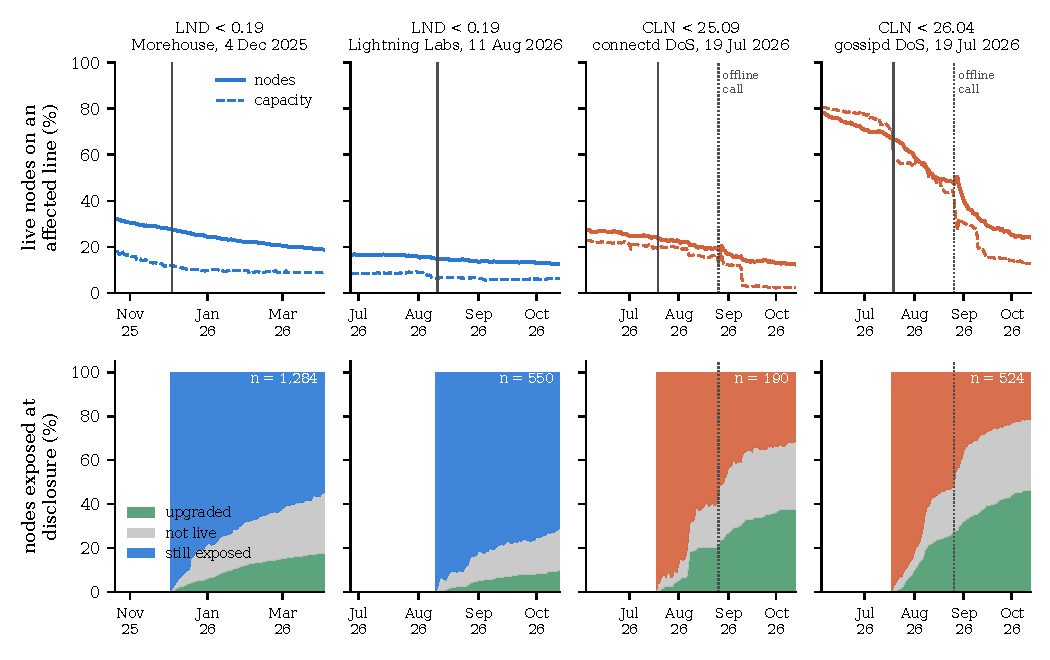
\includegraphics[width=\textwidth]{figures/fig6_exposure_cases.pdf}
\caption{Top: share of live nodes (solid) and of their live capacity (dashed) on a line affected by the advisory;
solid vertical line: disclosure; dotted: CLN's call of 26~August~2026 to upgrade or restart offline. Bottom: the nodes
exposed on the last snapshot before disclosure, by what became of them. Managed fleet excluded.}
\label{fig:cases}
\end{figure*}

% ==========================================================================================
\section{Discussion}
\label{sec:discussion}

\paragraph{Disclosure reaches the operators who were already upgrading}
The LND advisories of 2025 and 2026 were published long after the fixes shipped, a common practice that lets
operators upgrade before attackers learn what to look for. It works for the operators who follow releases: half of
LND nodes move to a new line within three months, and the largest move first. The nodes still on an affected line at
disclosure are the ones that did not, and the disclosure itself did not change their behaviour. Their upgrade rate in
the month after Lightning Labs' batch was the same as in the month before, and most of them were still exposed two
months later. Once a release is a year old, the exposed tail consists of nodes that upgrade rarely or never, which an
advisory alone does not reach. CLN's July disclosures did move operators: the rate at which nodes left vulnerable
lines rose two- to fourfold in the following month, before the maintainers' call of 26~August, after which exposure
fell further. We cannot separate the reasons. The fixed CLN lines were younger (one of the two fixes had shipped \FixToDiscClnGossipd{}
days before disclosure, against \FixToDiscLLBatch{} for LND), so more of the exposed operators were ones who usually keep up; CLN's
operators are fewer and closer to its maintainers; and its disclosures came amid an active run of CLN security
releases. Part of CLN's decline was nodes going offline rather than upgrading, which the maintainers asked for and
which also removes the exposure.

\paragraph{Platforms move nodes; size and attention keep them current}
Upgrades arrive in waves of a hundred or more nodes a few weeks after a release, consistent with node platforms
shipping updates to all their users at once, and one wave followed a merchant platform's security release within a
day. This matches what Frei et al.\ found for browsers: the update mechanism, more than the user, sets the patch
level~\cite{frei2009firefox}. The tail is the opposite population: small nodes, nodes that skipped earlier releases,
nodes no platform updates for them. For advisories that require a channel with the victim, these nodes are also the
cheapest to reach. Their share of capacity at risk is small (about \ExpCapLLBatchDisc\% for the August~2026 LND
batch), but each holds its operator's funds.

\paragraph{Counting nodes}
For half a year, one operator ran more than a fifth of the live LND nodes we observe, with almost no capacity. Any
statistic that counts nodes, whether implementation shares, version shares or exposure, would have been dominated by
that operator's choices. Fleets are cheap to create and hard to see; we found this one only because it upgraded in
step. Node-level Lightning measurements should look for such fleets before counting, and report capacity alongside
nodes~\cite{kumar2026clientdiversity}.

% ------------------------------------------------------------------------------------------
\section{Limitations}
\label{sec:limitations}
\emph{Release lines, not patches.} Gossip cannot separate patch releases, so fixes inside a line, including all
of CLN's 2026 patch releases, cannot be measured; for advisories with a fix inside a line we report bounds.
\emph{Inference.} An operator can switch features on or off so that an older line looks like a newer one or the
reverse; the strict range covers every non-developer configuration, and validation on self-identifying CLN nodes
bounds the error of the likely line, but we have no equivalent ground truth at scale for LND. A node that upgrades
without re-announcing, or whose announcement we do not receive, keeps its old bits, which biases exposure up.
\emph{Vantage and liveness.} All data come from one node's view of the public graph; unannounced nodes, including
most mobile wallets, are not covered, and liveness is inferred from peers' channel updates.
\emph{Fleets.} We identified one managed fleet by its alias and hubs. Smaller fleets without a shared alias would go
undetected and be counted as independent nodes.
\emph{Exposure is not exploitability.} Several advisories require a channel with the victim, a particular
configuration or inbound connections; we count nodes on affected releases, not nodes that can be attacked. Our
advisory list is compiled from public sources and may miss silent fixes.
\emph{Association.} The hazard model describes which nodes upgrade sooner; it does not identify why.

% ------------------------------------------------------------------------------------------
\section{Ethics}
\label{sec:ethics}
Release-line inference identifies nodes running vulnerable software, and in 2026 Lightning deployments were
exploited (BTCPay Server~\cite{btcpay2026advisory}) and CLN maintainers reported attacks on unpatched nodes. We therefore publish aggregates only: no list, ranking, filter or label of
individual nodes by release or exposure, in the paper or in the released data. All inputs are public gossip,
every advisory we study had been published before our analysis began, and the paper reports no new vulnerability.

% ------------------------------------------------------------------------------------------
\section{Conclusion}
\label{sec:conclusion}
Lightning gossip carries no version string, but the feature bits each release announces identify its release line
closely enough to measure how the network patches. Most operators upgrade within a few months, in waves pushed by
their platforms; a tail of small and neglected nodes does not, and LND's disclosures, which typically come long after
the fix, leave that tail where it was. CLN's 2026 disclosures, followed by the maintainers' appeal, moved theirs. Measured by capacity, the
exposure is small; measured by nodes, it depends on whether one counts a single operator's fleet as hundreds of
operators.


\section*{Data and Code Availability}
Code, the aggregate datasets behind every figure and table, and a script that recomputes every number quoted in the
text are available at \url{https://github.com/bitcoindatalabs/ln-upgrade-dynamics}. All stages truncate their inputs
at the data cutoff of 13~October~2026. The underlying gossip data are public; our daily gossip snapshots are
available from the author on request.

\bibliographystyle{IEEEtran}
\bibliography{references}

\end{document}
